% -----------------------------------------------
% Template for SMAC SMC 2013
% adapted from the template for SMC 2012, which was adapted from that of SMC 2011
% -----------------------------------------------

\documentclass{article}
\usepackage{smacsmc2013}
\usepackage[utf8]{inputenc}
\usepackage{times}
\usepackage{ifpdf}
\usepackage[english]{babel}
\usepackage{cite}
\usepackage{color}

%%%%%%%%%%%%%%%%%%%%%%%% Some useful packages %%%%%%%%%%%%%%%%%%%%%%%%%%%%%%%
%%%%%%%%%%%%%%%%%%%%%%%% See related documentation %%%%%%%%%%%%%%%%%%%%%%%%%%
%\usepackage{amsmath} % popular packages from Am. Math. Soc. Please use the 
%\usepackage{amssymb} % related math environments (split, subequation, cases,
%\usepackage{amsfonts}% multline, etc.)
%\usepackage{bm}      % Bold Math package, defines the command \bf{}
%\usepackage{paralist}% extended list environments
%%subfig.sty is the modern replacement for subfigure.sty. However, subfig.sty 
%%requires and automatically loads caption.sty which overrides class handling 
%%of captions. To prevent this problem, preload caption.sty with caption=false 
%\usepackage[caption=false]{caption}
%\usepackage[font=footnotesize]{subfig}


%user defined variables
\def\papertitle{Programming Interactive Music Scores with INScore}
\def\firstauthor{D. Fober}
\def\secondauthor{S. Letz}
\def\thirdauthor{Y. Orlarey}

% adds the automatic
% Saves a lot of ouptut space in PDF... after conversion with the distiller
% Delete if you cannot get PS fonts working on your system.

% pdf-tex settings: detect automatically if run by latex or pdflatex
\newif\ifpdf
\ifx\pdfoutput\relax
\else
   \ifcase\pdfoutput
      \pdffalse
   \else
      \pdftrue
\fi

\ifpdf % compiling with pdflatex
  \usepackage[pdftex,
    pdftitle={\papertitle},
    pdfauthor={\firstauthor, \secondauthor, \thirdauthor},
    bookmarksnumbered, % use section numbers with bookmarks
    pdfstartview=XYZ % start with zoom=100% instead of full screen; 
                     % especially useful if working with a big screen :-)
   ]{hyperref}
  %\pdfcompresslevel=9

  \usepackage[pdftex]{graphicx}
  % declare the path(s) where your graphic files are and their extensions so 
  %you won't have to specify these with every instance of \includegraphics
  \graphicspath{{./figures/}}
  \DeclareGraphicsExtensions{.pdf,.jpeg,.png}

  \usepackage[figure,table]{hypcap}

\else % compiling with latex
  \usepackage[dvips,
    bookmarksnumbered, % use section numbers with bookmarks
    pdfstartview=XYZ % start with zoom=100% instead of full screen
  ]{hyperref}  % hyperrefs are active in the pdf file after conversion

  \usepackage[dvips]{epsfig,graphicx}
  % declare the path(s) where your graphic files are and their extensions so 
  %you won't have to specify these with every instance of \includegraphics
  \graphicspath{{./figures/}}
  \DeclareGraphicsExtensions{.eps}

  \usepackage[figure,table]{hypcap}
\fi

%setup the hyperref package - make the links black without a surrounding frame
\hypersetup{
    colorlinks,%
    citecolor=black,%
    filecolor=black,%
    linkcolor=black,%
    urlcolor=black
}


% Title.
% ------
\title{\papertitle}

% Authors
% Please note that submissions are NOT anonymous, therefore 
% authors' names have to be VISIBLE in your manuscript. 
%
% Single address
% To use with only one author or several with the same address
% ---------------
%\oneauthor
%   {Dominique Fober, Stéphane Letz, Yann Orlarey} {\textsc{Grame} \\ %
%   	Centre National de Création Musicale \\
%	Lyon - France\\
%   {\tt \href{mailto:fober@grame.fr}{fober@grame.fr} 
%     \href{mailto:letz@grame.fr}{letz@grame.fr}
%     \href{mailto:orlarey@grame.fr}{orlarey@grame.fr}}}

%Two addresses
%--------------
% \twoauthors
%   {\firstauthor} {Affiliation1 \\ %
%    {\tt \href{mailto:author1@smcnetwork.org}{author1@smcnetwork.org}}}
%   {\secondauthor} {Affiliation2 \\ %
%     {\tt \href{mailto:author2@smcnetwork.org}{author2@smcnetwork.org}}}


 \twoauthors
   {D. Fober, S. Letz, Y. Orlarey} {\textsc{Grame} \\
%	Centre National de Création Musicale \\
	Lyon - France \\
   {{\small \tt \href{mailto:fober@grame.fr}{fober}, 
     \href{mailto:letz@grame.fr}{letz},
     \href{mailto:orlarey@grame.fr}{orlarey}@grame.fr}}}
   {F. Bevilacqua} {\textsc{IRCAM} \\ %
	Paris - France \\
     {{\small \tt \href{mailto:Frederic.Bevilacqua@ircam.fr}{Frederic.Bevilacqua@ircam.fr}}}}

% Three addresses
% --------------
% \threeauthors
%   {\firstauthor} {Affiliation1 \\ %
%     {\tt \href{mailto:author1@smcnetwork.org}{author1@smcnetwork.org}}}
%   {\secondauthor} {Affiliation2 \\ %
%     {\tt \href{mailto:author2@smcnetwork.org}{author2@smcnetwork.org}}}
%   {\thirdauthor} { Affiliation3 \\ %
%     {\tt \href{mailto:author3@smcnetwork.org}{author3@smcnetwork.org}}}



% ------------------------------------------------
\definecolor{mygrey}			{gray}{0.93}
\newcommand{\inscore}		{\textsc{\small INScore}}
\newcommand{\code}[1]		{\texttt{\small #1}}

\newcounter{excount}
\setcounter{excount}{1}
\newcommand{\exemple}			{\vspace{1mm} \hspace*{-4.5mm}\textbf{Example \arabic{excount}} \addtocounter{excount}{1}}
\newcommand{\sample}	[1]		{\begin{center}\colorbox{mygrey}{
								\begin{minipage}[t]{0.95\columnwidth} 
								{\small \texttt{#1}}
								\end{minipage}}\end{center}}

% ***************************************** the document starts here ***************
\begin{document}
%
\capstartfalse
\maketitle
\capstarttrue
%
\begin{abstract}
\inscore\ is an environment for the design of interactive music scores that includes an original event-based interaction system and a scripting language for associating arbitrary messages to these events. We extended the previous version by supporting scripting languages offering a great flexibility in the description of scores and in the interactions with scores. The textual format is directly derived from the OSC message format that was defined in the original \inscore\ version. This article presents the scripting language and illustrates its ability to describe interactions based on events, while remaining in the temporal space. It also introduces the IRCAM gesture follower and how it is embedded into \inscore\ to provide gestural interaction capabilities.
\end{abstract}
%

\section{Introduction}\label{sec:introduction}
\inscore\ is a dynamic music score viewer that can be controlled in real-time via OSC messages as well as using OSC based scripts. It supports extended music scores \cite{Fober:10c}, combining symbolic notation with arbitrary graphic objects. All the objects of a score have a time dimension and can be synchronized in a master/slave relationship i.e. any object can be placed in the time space of another object \cite{Fober:10b}. 
It can be used in concert, notably for interactive music pieces, for music analysis, for pedagogical applications, etc.

%\inscore\ is an environment for the design of musical scores that proposes an approach to musical notation extended to arbitrary graphical objects \cite{Fober:10c}, including the representation of musical interpretation. This new approach of music notation also supports the representation of the temporal relations between the objects of the score \cite{Fober:10b}.

\inscore\ has been designed in response to a lack of computer tools for music notation, which did not evolved in proportion to the new forms of musical creation (see eg \cite{magnuss11} \cite{freeman11}).
In particular, there is a significant gap between interactive music and the way it is statically written.
%================================
%================================

Music notation generated in interaction with live performance exists for more than a decade. As mentioned by Freeman \cite{Freeman:2008:ESM:1403124.1403129}, numerous approaches exist: selection of pre-determined score excerpts \cite{Kim-Boyle:2005:MSG:1085939.1086007}, mixture of symbolic and graphic elements \cite{winkler2004}, use of unconventional graphical notation \cite{Gutknecht:2005:GUR:1085939.1085980}, complex staff based notation \cite{didkovsky2004recent}. 

These works are based on custom tools, sometimes designed using Max, that are generally specifically suited to a composer approach. Didovsky used JMSL \cite{didkovsky2001java} to design interactive scores, but JMSL should be considered more as a programming language for Java applications developers than an environment for composers. Baird is using Lilypond \cite{lilypond03} for audience interaction \cite{Baird:2005:RGM:1085939.1086008}, that can't be considered as a real-time environment for generating music scores, although it works in Baird's context due to relaxed time constraints.

With the recent Bach \cite{agostini12b} or MaxScore \cite{didko08} environments, the symbolic dimension of the music notation starts to be accessible to interaction, first using Max and next the Live environment. However, they are not designed to support unconventional graphical notation, although it could be implemented in Max using Jitter for example.

A unified environment, covering symbolic and graphic notation, opened to real-time interaction is missing and \inscore\ aims at fulfilling the needs emerging from the contemporary creation. 

%but the symbolic dimension of the notation is generally excluded from the interaction process except in recent works \cite{Hoadley12}. 

%================================
%================================
Designed to be controlled by OSC messages, \inscore\ is naturally turned to an interactive use. The approach to music score programming is also supported by a scripting language based on an extension of the OSC messages, and providing interaction primitives based on \emph{events}. These events are similar to those typically available for user interfaces management (e.g. via Javascript DOM \cite{dom3ev}), with an extension in the time domain.

The next section shows two examples of interactive scores, implemented in recent creations using \inscore. Then it presents the message system and the interaction events, that allow both to describe the music score and to interact with it. Examples of uses are finally given, to illustrate the expressive capabilities of the system.


\section{Interactive Music Scores}\label{interactscore}

Today, interactive music is subject of convergent artistic and scientific interests. Interaction raises issues for the artistic work composition, description and performance as well.
These issues are addressed in the temporal aspects of interactive scores \cite{allombert09} 
or control \cite{acont08}, and are related to the music piece computation.

For interactive pieces notation, two recent works have used \inscore\ to create dynamic scores with original approaches, that also reflect the needs of the contemporary music creation. These works are \emph{Calder's Violin} and \emph{Alien Lands}.

\subsection{Calder's Violin}
\textit{Calder's violin}, composed by Richard Hoadley, has been created in Cambridge in October 2011. The piece is defined as a composition for violin and automatic piano. Dynamic symbolic music notation is generated algorithmically and presented to the musician (figure \ref{fig:cv}) in real-time. This score is played by the musician in parallel to sounds generated by the computer. 
The technological environment includes SuperCollider for the audio programming and \inscore\ for the music notation. For more details, you can refer to \cite{Hoadley12}. 

\begin{figure}[htbp]
\centerline{
	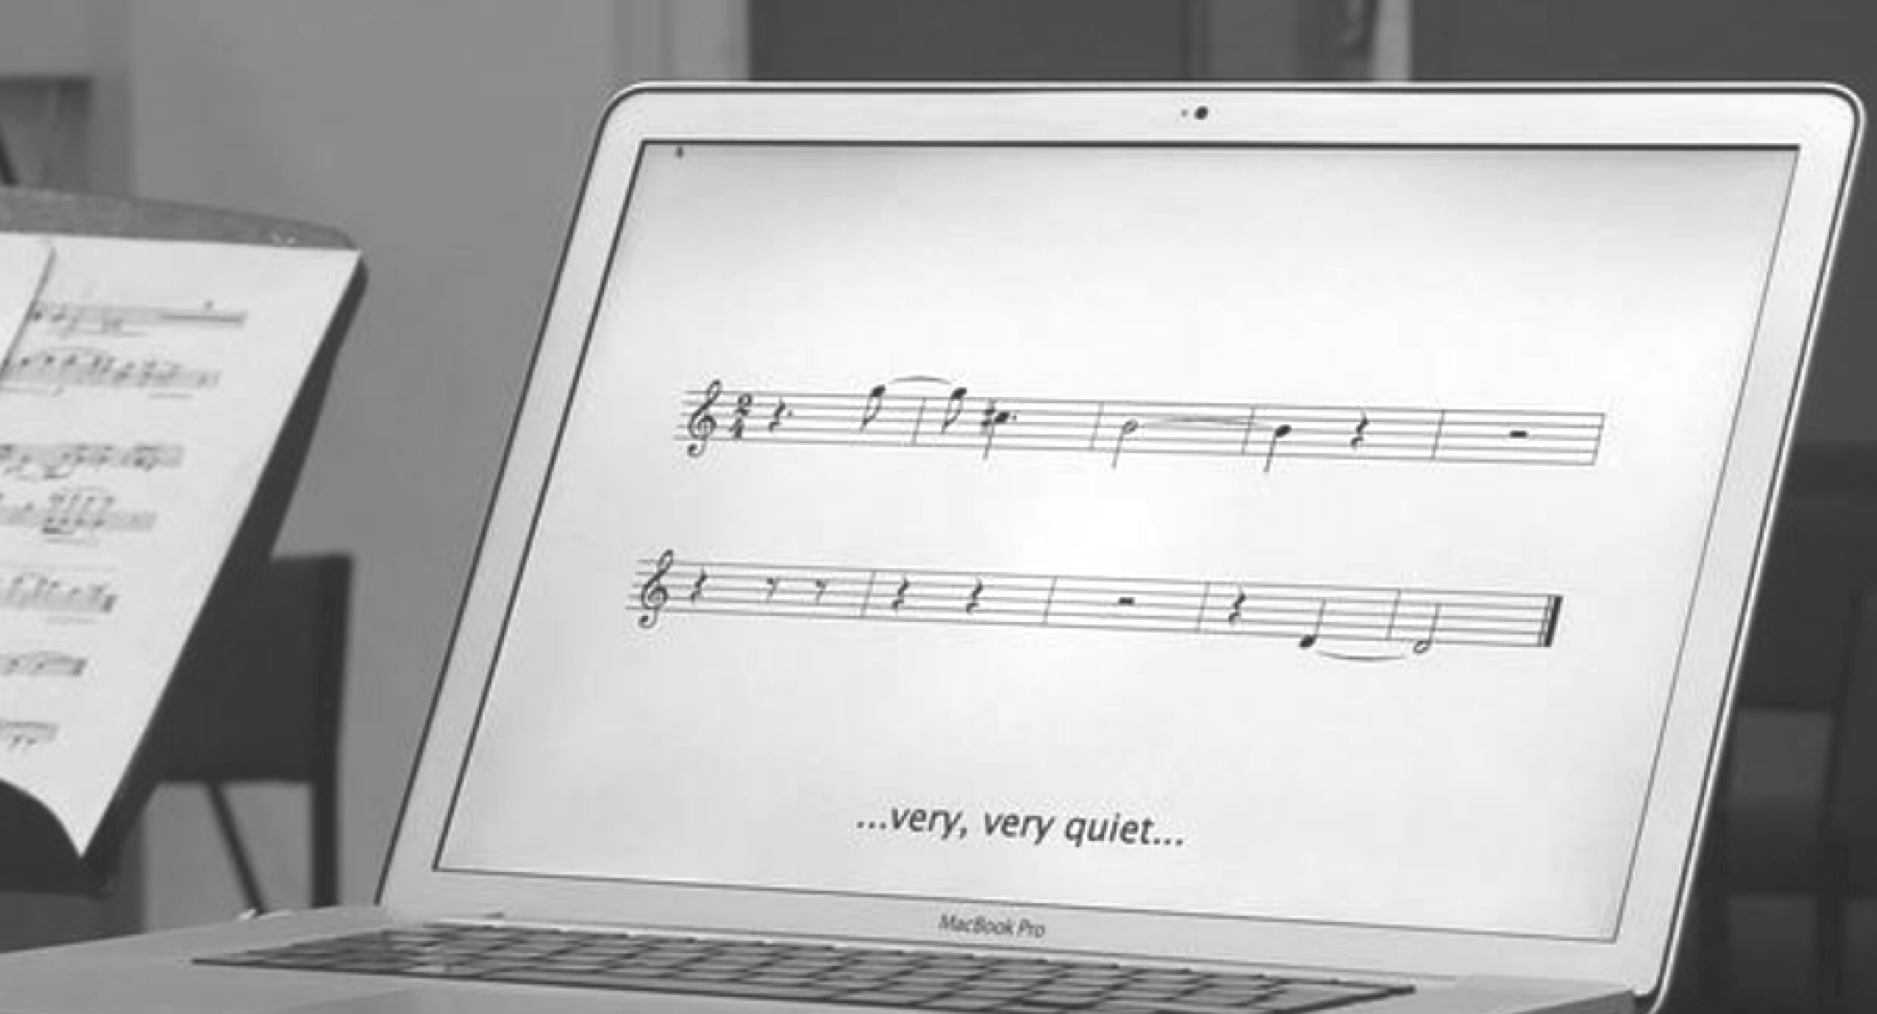
\includegraphics[width=0.9\columnwidth]{imgs/caldersv}}
\caption{Calder's Violin: sample of music notation.}
\label{fig:cv}
\end{figure}

\subsection{Alien Lands}

\textit{Alien Lands} is a set of pieces for percussions and string quartet, composed by Sandeep Bhagwati. 
The interactive version of the pieces has been given in Montreal in February 2011.
Use of \inscore\ falls in 4 categories:
\begin{itemize}
\item traditional music score with automatic page turning,
\item music score including automatic choices made by the computer: order of the measures, staves selection,
\item complex automatic music score, including elements generated algorithmically (figure \ref{fig:al}),
\item complex interactive music score, where the dynamic element are generated at musician request.
\end{itemize}

\begin{figure}[htbp]
\centerline{
	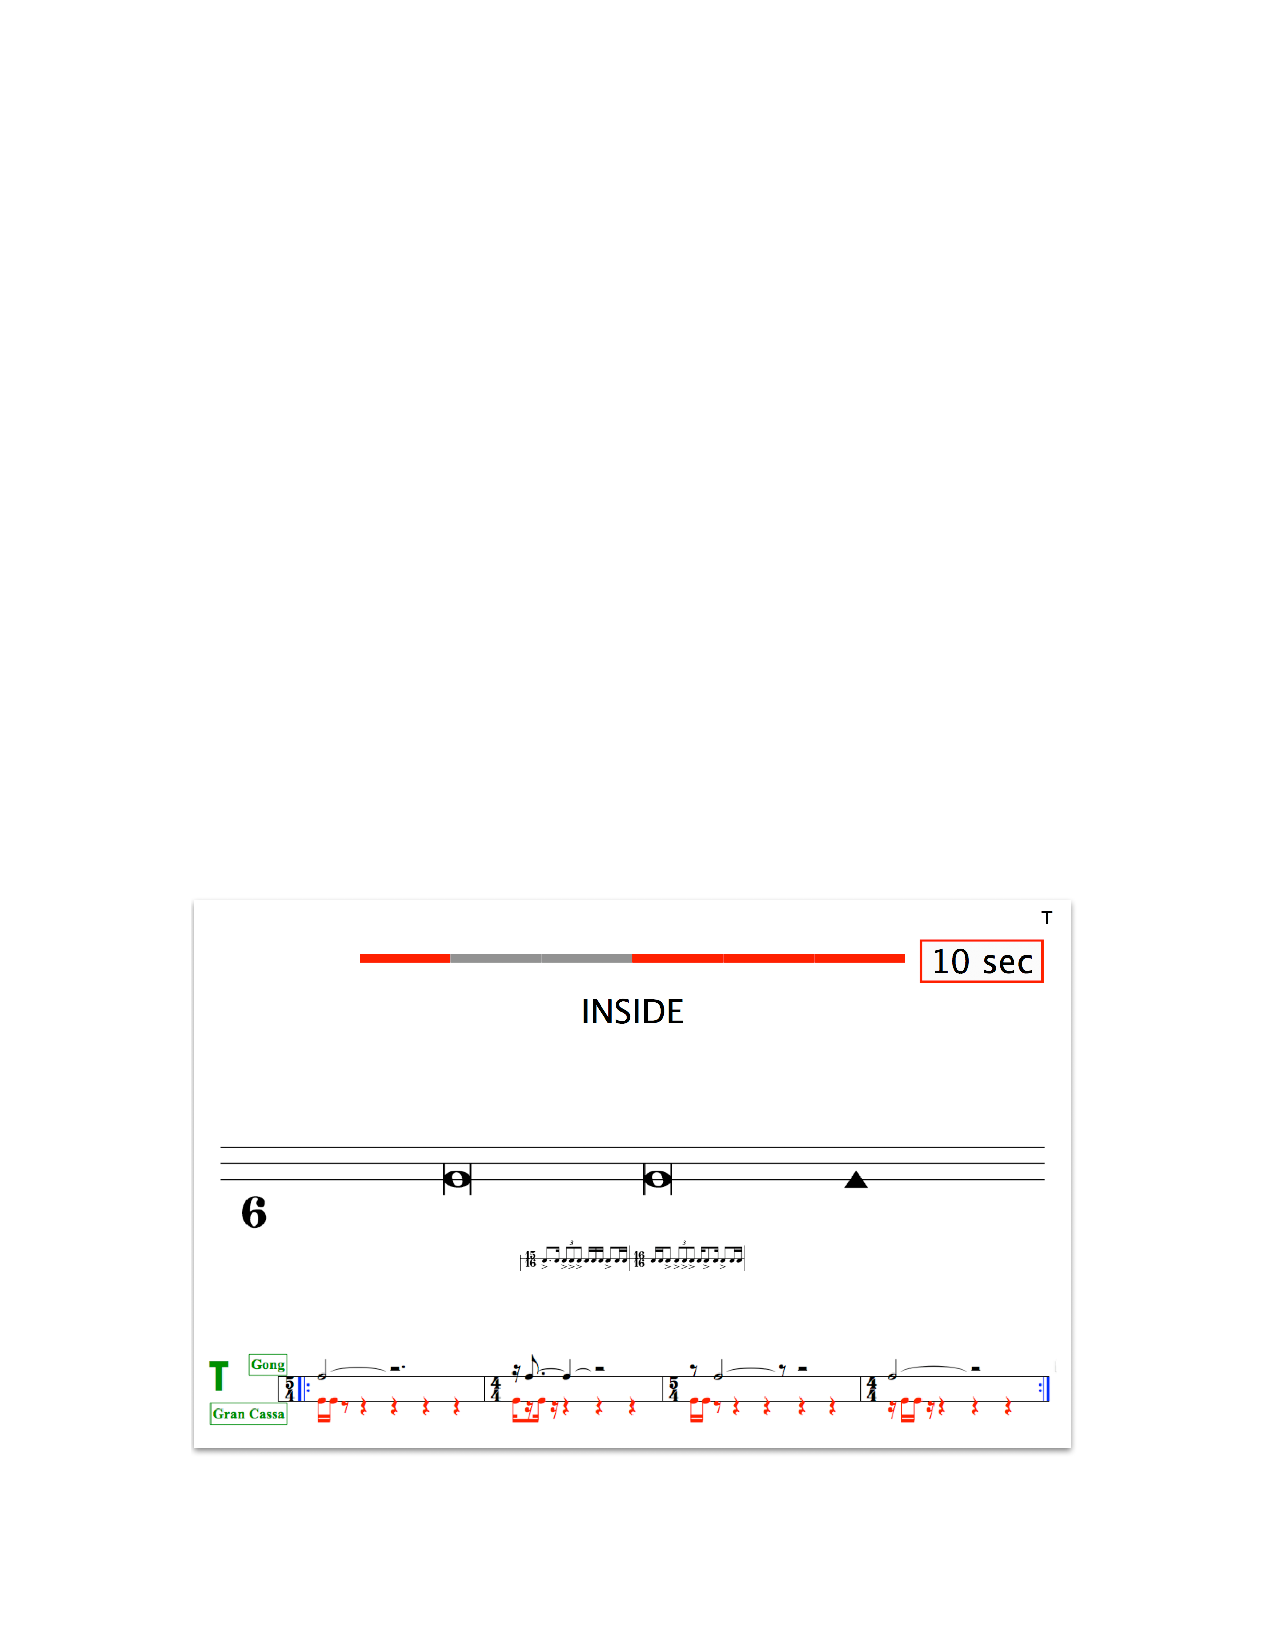
\includegraphics[width=0.94\columnwidth]{imgs/alienscore}}
\caption{Alien Lands : a complex automatic music score.}
\label{fig:al}
\end{figure}

%----------------------------------------------
\section{Music score design using messages}\label{sec:msgs}

The basic principle for the description of a music score consists in sending OSC messages to the system to create the different score components and to control their attributes, both in graphic and time spaces.

%========================
\subsection{Format of the messages}
The global format of the \inscore\ messages is illustrated in figure \ref{fig:fgal} in a syntax diagram specified in EBNF. It consists in a specialization of the OSC specification that may be viewed as \emph{object oriented}, where the address indicates the target object of the message, \code{method} indicates a method of the target object and \code{params}, the method parameters. An \inscore\ message could be viewed as a method call of an object of the score.

\begin{figure}[htbp]
\centerline{
	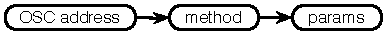
\includegraphics[width=0.8\columnwidth]{imgs/formatgal}}
\caption{Format of the INScore messages.}
\label{fig:fgal}
\end{figure}

The system includes messages to control the objects graphical attributes (position, color, scale, rotation, effects ...) to control their temporal attributes (date, time), to express the relationship between graphic and time spaces, to synchronize different score components, to draw \emph{graphic} signals, and to manage interaction events.

\exemple \\
Changing the \code{x} position of an object named \code{obj}. The address describes the objects hierarchy: \code{obj} is embedded in a score named \code{scene} that is included in the application which address is \code{ITL}.
\vspace{-1mm}\sample{/ITL/scene/obj x -0.5}


%========================
\subsection{Scripting}

Although intended to be sent as packets over a network, the OSC messages can be expressed under a textual form, which constitutes the file storage format of a score. This textual form has been extended to enforce the scripting capabilities of the system. The \inscore\ viewer supports loading or drag \& drop of scripts files, which is equivalent to send the enclosed or evaluated OSC messages to the system.

\subsubsection{Extended adresses}

The OSC addresses have been extended to support targeting external applications and/or stations (Figure \ref{fig:eaddr}). It allows to initialize both the music score and external resources as well using the same script.

\begin{figure}[htbp]
\centerline{
	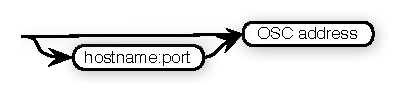
\includegraphics[width=0.8\columnwidth]{imgs/extaddress}}
\caption{Addressing scheme extension.}
\label{fig:eaddr}
\end{figure}

\exemple \\
Initializes a score with a Guido Music Notation file\cite{hoos98} and sends a message to an external application listening on port \code{12000} on a station named \code{host.adomain.net}. The semicolon (;) is used as a message terminator in a script.
\vspace{-1mm}\sample{/ITL/scene/score set gmnf 'myscore.gmn'; \\
host.adomain.net:12000/run 1; }

\subsubsection{Variables}

Variables have been introduced to allow sharing of parameters between messages. A variable associates an identifier and a parameter list or a list of messages (Figure \ref{fig:var}). Variables can be used as message parameter using the form \code{\$identifier}.

\begin{figure}[htbp]
\centerline{
	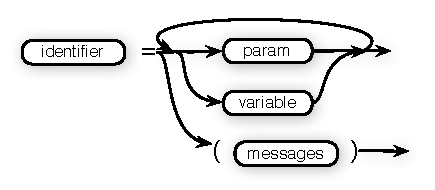
\includegraphics[width=0.8\columnwidth]{imgs/variables}}
\caption{Variables.}
\label{fig:var}
\end{figure}

\exemple \\
Variable declaration and use. The exclamation point (!) starts a line comment.
\vspace{-1mm}\sample{color = 200 200 200; \\
! using the previous color variable\\
colorwithalpha = \$color 100;  \\
/ITL/scene/obj color \$colorwithalpha;
 }

\subsubsection{Languages}

\inscore\ scripts support programming languages like java-script (default) or lua. The corresponding sections are indicated by angle brackets as in html (Figure \ref{fig:lang}). The code is evaluated at parse time and the output of the evaluation should be a set of \inscore\ messages that will be next parsed in place of the corresponding section.

\begin{figure}[htbp]
\centerline{
	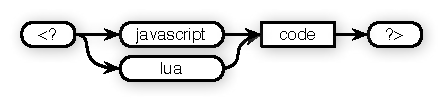
\includegraphics[width=0.8\columnwidth]{imgs/scripts}}
\caption{Languages.}
\label{fig:lang}
\end{figure}

%----------------------------------------------
\section{Events based interaction}\label{sec:interaction}

Interaction is based on associations between events and messages. The messages are sent when the event occurs. The general format of the messages to create such associations is described in Figure \ref{fig:watch}.

\begin{figure}[htbp]
\centerline{
	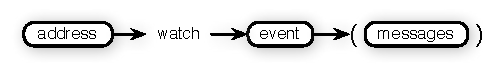
\includegraphics[width=0.95\columnwidth]{imgs/watch}}
\caption{Format of an interaction message.}
\label{fig:watch}
\end{figure}

%----------------------------------------------
\subsection{Events typologie}\label{subsec:typologie}

Events defined by the system are basically 1) typical user interface events (e.g. mouse click and mouse move) and 2) events defined in the time domain (table \ref{tbl:evts}). This typology has been extended to \emph{gesture events}, described in section \ref{sec:gev}.

\begin{table}[htdp]
\begin{center}
\begin{tabular}{c|c}
Graphic domain & Time domain \\
\hline
mouseDown 		& timeEnter	\\
mouseUp			& timeLeave	\\
mouseEnter		& durEnter		\\
mouseLeave		& durLeave		\\
mouseMove		&				\\
\end{tabular}
\end{center}
\caption{Main events of the system.}
\label{tbl:evts}
\end{table}%

In the time domain, an event is triggered when an object date enters (\code{timeEnter}) or leaves (\code{timeLeave}) a time interval defined by 2 dates, or when an object duration enters (\code{durEnter}) or leaves (\code{durLeave}) an interval bounded by 2 durations.

%----------------------------------------------
\subsection{Contextual variables}
A \emph{contextual variable} is a variable which value depends on an event context (unlike script variables that are evaluated when loading the script). 
Most of these variables concern the graphic domain and are associated to user interface events; they give the mouse position at the time of the event occurrence and expressed in different reference spaces (\code{\$x \$y \$sx \$sy}). A variable can also give the date corresponding to the current mouse position (\code{\$date}).
When an event occurs, the associated messages are evaluated because they may refer to contextual variables. 

\exemple  \\ Asking an object to follow the mouse down. The comma (,) is used as separator in a messages list.
\sample{/ITL/scene/obj watch mouseDown (\\
\hspace*{12mm}/ITL/scene/obj x '\$sx', \\
\hspace*{12mm}/ITL/scene/obj y '\$sy' );}


%----------------------------------------------
\subsection{Managing interaction states}
Every score component includes a stack to store interaction states. The methods \code{push} and \code{pop} are provided to push the current interaction state to the stack and to pop and restore a state from the top of the stack. Examples are given in section \ref{seqloop}.



%----------------------------------------------
\section{Use cases}\label{sec:exemples}


%----------------------------------------------
\subsection{Page turning} \label{pageturn}

A simple use case consists in automatic page turning. An object can watch the time intervals corresponding to the different pages and recall a page when it enters its time interval. Time is specified in music time where 1 is a whole note. Note that the \code{obj} object could be a cursor moving on the score as well.
\sample{! first page duration is 12 whole notes
/ITL/scene/obj watch timeEnter 0 12	\\
\hspace*{25mm}(/ITL/scene/score page 1);	\\
/ITL/scene/obj watch timeEnter 12 24	\\
\hspace*{25mm}(/ITL/scene/score page 2);	\\
\hspace*{1mm}etc.
}


%----------------------------------------------
\subsection{Sequence of interactions} \label{seqitl}

Interaction messages described in figure \ref{fig:watch} accept arbitrary messages to be associated to an event. Thus it is possible to associate an interaction message to an event and to describe sequences of interaction.

\exemple   \\
Decription of an interaction sequence based  on mouse clicks: the first click changes the object color, the second affects the scaling, the third rotates the object, the fourth modifies the scale too... 
\sample{/ITL/scene/obj watch mouseDown ( 		\\
\hspace*{4mm}/ITL/scene/obj color 100 100 255,	\\
\hspace*{4mm}/ITL/scene/obj watch mouseDown (		\\
\hspace*{8mm}/ITL/scene/obj scale 1.4,			\\
\hspace*{8mm}/ITL/scene/obj watch mouseDown ( \\
\hspace*{12mm}/ITL/scene/obj angle 45. ,	 \\
\hspace*{12mm}/ITL/scene/obj watch mouseDown ( \\
\hspace*{16mm}/ITL/scene/obj scale 0.8 ))));
}

%----------------------------------------------
\subsection{Looping a sequence of interactions} \label{seqloop}
A sequence of interactions can be executed n times using the \code{push} and \code{pop} methods.

\exemple \\
Executing a sequence of 2 interactions 3 times.
\sample{/ITL/scene/obj watch mouseDown ( 		\\
\hspace*{4mm}/ITL/scene/obj color 255 0 0,	\\
\hspace*{4mm}/ITL/scene/obj watch mouseDown (		\\
\hspace*{8mm}/ITL/scene/obj color 0 0 255,	\\
\hspace*{8mm}/ITL/scene/obj pop ))	\\
/ITL/scene/obj push; \\
/ITL/scene/obj push;
} 

\exemple \\
Executing a sequence of 2 interactions in an infinite loop.
\sample{/ITL/scene/obj watch mouseDown ( 		\\
\hspace*{4mm}/ITL/scene/obj push,	\\
\hspace*{4mm}/ITL/scene/obj color 255 0 0,	\\
\hspace*{4mm}/ITL/scene/obj watch mouseDown (		\\
\hspace*{8mm}/ITL/scene/obj color 0 0 255,	\\
\hspace*{8mm}/ITL/scene/obj pop ))	\\
} 


%----------------------------------------------
\subsection{Interaction in the time domain}

The sequence of interactions described above (section \ref{seqitl}) could be defined in the time domain using associations between messages and time events and by moving the object in time. With this approach, it is possible to access the events in a random order but also to control the time flow of the events.

This kind of description combines event based approach, non-sequential access and temporal control.

\exemple   \\
Description of an interaction sequence using time events that are triggered when the object enters consecutives time zones, which duration is a whole note.
\sample{/ITL/scene/obj watch timeEnter 1 2	\\
\hspace*{10mm}(/ITL/scene/obj color 100 100 255);	\\
/ITL/scene/obj watch timeEnter 2 3	\\
\hspace*{10mm}(/ITL/scene/obj scale 1.4);	\\
/ITL/scene/obj watch timeEnter 3 4	\\
\hspace*{10mm}(/ITL/scene/obj angle 45.);	\\
/ITL/scene/obj watch timeEnter 4 5	\\
\hspace*{10mm}(/ITL/scene/obj scale 0.8);
}


%----------------------------------------------
\section{Interaction with gestures}\label{sec:igf}

\inscore\ may embed the IRCAM gesture follower as an external plugin. The corresponding objects are similar to signals from input viewpoint. They provide specific interaction events and may also generate streams of messages.

%-------------------------
\subsection{Principle of the gesture follower}\label{sec:pgf}
The IRCAM gesture follower if a tool to perform template-based recognition \cite{bevilacqua10,Bevilacqua2011}. Technically, the algorithm is available as a C++ library that can be implemented in various environments (up to now the  objet called \emph{gf} was the most common instantiation of the library in the Max environment). The gestures can be any type of temporal multidimensional times series, that must be regularly time-sampled. Typically, a drawing is a two-dimensional signal, but other signal types can be used such as three, six or nine dimension data obtained from inertial measurement units.

The gesture follower, as most recognition system, is based on two steps. The first step, called \emph{learning}, corresponds to setting a series of "templates". Each template is used to set a Markov Chain modeling the times series. The second step, called  \emph{following}, corresponds to "compare" incoming data flow with the stored templates. Technically, the decoding is based on the forward procedure to estimate \emph{likelihoods} of the incoming data to match each templates (note that the forward procedure is incremental compared to a standard Viterbi algorithms). The gesture follower also outputs  the \emph{position} (or \emph{temporal index}) that is an estimation of the corresponding current position within the templates, and the estimated \emph{speed} (relative to their templates).

%-------------------------
\subsection{Gesture follower object}\label{sec:gfo}

Provided that the corresponding plugin is available, a \emph{gesture follower} object may be embedded in a score. It is created with a fixed set of named gestures to be recognized and thus, its address space is automatically extended to the set of named gestures.

\exemple \\
Address space of a gesture follower named \emph{myFollower} created to handle 2 gestures named \emph{gestureA} and \emph{gestureB}
\sample{/ITL/scene/myFollower \\
/ITL/scene/myFollower/gestureA \\
/ITL/scene/myFollower/gestureB
}

A gesture follower may take 3 states: a learning state, a following state and an idle state. It receives values that are stored to the corresponding gesture when in learning state, analysed to recognize a gesture when in following state and ignored when idle. Each time the follower receives data in the following state, it produces a set of likelihood, position and speed for each of the gestures.

%-------------------------
\subsection{Gestures events}\label{sec:gev}
Specific events are available from gestures and depends on the gesture state. A gesture may be \emph{active} or \emph{idle}: it is active when its likelihood is greater or equal than a given threshold, otherwise it is idle (figure \ref{fig:geststates}). 

\begin{figure}[htbp]
\centerline{
	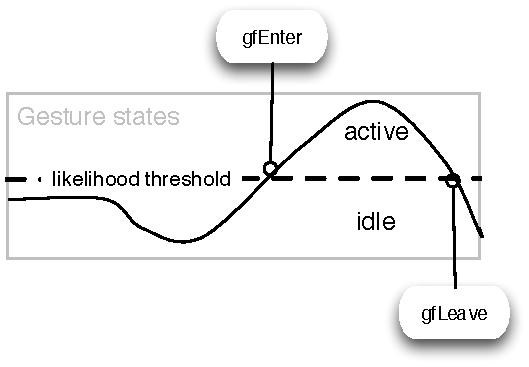
\includegraphics[width=0.6\columnwidth]{imgs/geststates}}
\caption{A gesture states and events.}
\label{fig:geststates}
\end{figure}

Two specific events are associated to gestures :
\begin{itemize}
\item \code{gfEnter}: triggered when a gesture state moves from idle to active,
\item \code{gfLeave}: triggered when a gesture state moves from active to idle.
\end{itemize}


%-------------------------
\subsection{Gesture streams}\label{sec:gestream}

A gesture supports messages streaming, depending on its state. Figure \ref{fig:gestream} presents the \code{send} method that associates a list of messages to the \code{active} or \code{idle} state of a gesture. The messages are sent when the gesture follower state is refreshed i.e. when it is in following mode and each time it receives data.

\begin{figure}[htbp]
\centerline{
	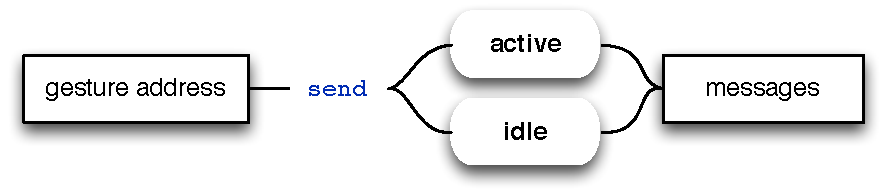
\includegraphics[width=0.9\columnwidth]{imgs/gestream}}
\caption{Associating messages to gesture states.}
\label{fig:gestream}
\end{figure}

%-------------------------
\subsection{Variables defined in the context of gestures}\label{sec:gesvar}

Specific variables may be used by messages associated to gesture events or streams:
\begin{itemize}
\item \code{\$likelihood} : gives the current gesture likelihood,
\item \code{\$pos} : indicates the current position in the gesture,
\item \code{\$speed} : indicates the current speed of the gesture.
\end{itemize}
These variables support scaling and translation of their values when suffixed using an interval. The values denoted by \code{\$pos[1,5]} represents the current position scaled between 1 and 5.

\exemple \\
Using a gesture to move a cursor date from 0 to 1.
\sample{/ITL/scene/gf/gesture send active \\
\hspace*{1.5cm}(/ITL/scene/cursor date \$pos);
}

\section{Conclusion}

Using the OSC protocol to design a scripting language constitutes an original approach which is simple to apprehend for people familiar with OSC. While none of classical programming languages constructs exists in \inscore\ scripts, programming capabilities emerge from the objects behavior and leads to new conceptions of music score design. 

The association of messages to events reveals to be a simple, powerful and homogeneous way to describe dynamic music scores. A single textual script serves the need of both the static and dynamic parts of the score, leading to new kind of programming e.g. moving of objects in the time domain using an external application when these objects are designed using behaviors linked to time intervals. 

This system opens a new dimension to the score components that were previously passive objects: they could react to messages but didn't send messages by themselves. While becoming active and able to send messages, autonomous dynamic behaviors emerge and since each object may embed its own behavior, the system may be viewed as a parallel programmable music score.

However, an external application or the user interaction is necessary to move objects in time. This is currently not considered as a limitation since external applications remain also necessary for the music itself.

%
\begin{acknowledgments}
This research has been conducted in the framework of the INEDIT project that is funded by the French National Research Agency [ANR-12-CORD-009-03].
\end{acknowledgments} 

%%%%%%%%%%%%%%%%%%%%%%%%%%%%%%%%%%%%%%%%%%%%%%%%%%%%%%%%%%%%%%%%%%%%%%%%%%%%%
%bibliography here
\bibliography{../interlude}

\end{document}
